% -*- TeX:UTF-8 -*-
%%
%% KAIST 학위논문양식 LaTeX용 (ver 0.4) 예시
%%
%% @version 0.4
%% @author  채승병 Chae,Seungbyung (mailto:chess@kaist.ac.kr)
%% @date    2004. 11. 12.
%%
%% @requirement
%% teTeX, fpTeX, teTeX 등의 LaTeX2e 배포판
%% + 은광희 님의 HLaTeX 0.991 이상 버젼 또는 홍석호 님의 HPACK 1.0
%% : 설치에 대한 자세한 정보는 http://www.ktug.or.kr을 참조바랍니다.
%%
%% @note
%% 기존에 널리 쓰여오던 차재춘 님의 학위논문양식 클래스 파일의 형식을
%% 따르지 않고 전면적으로 다시 작성하였습니다. 논문 정보 입력부분에서
%% 과거 양식과 다른 부분이 많으니 아래 예시에 맞춰 바꿔주십시오.
%%
%%
%% @acknowledgement
%% 본 예시 논문은 물리학과 박사과정 김용현 님의 호의로 제공되었습니다.
%%
%% -------------------------------------------------------------------
%% @information
%% 이 예제 파일은 hangul-ucs를 사용합니다. UTF-8 입력 인코딩으로
%% 작성되었습니다. hlatex의 hfont는 이용하지 않습니다. --2006/02/11
%% 본 템플릿은 전산학부 김민혁 교수에의해서 버그 수정되었습니다. -- 2016/11/25
%% 본 템플릿은 전산학부 김민혁 교수에의해서 추가 버그 수정되었습니다. -- 2023/06/15

% @class kaist.cls
% @options [default: doctor, korean, final]
% - doctor: 박사과정 | master : 석사과정
% - korean: 한글논문 | english: 영문논문
% - final : 최종판   | draft  : 시험판
% - pdfdoc : 선택하지 않으면 북마크와 colorlink를 만들지 않습니다.


%\documentclass[master,korean,final]{kaist-ucs} % 석사과정
% \documentclass[doctor,korean,final]{kaist-ucs} % 박사과정
\documentclass[master,english,final]{kaist-ucs} % 박사과정

% If you want make pdf document (include bookmark, colorlink)
%\documentclass[doctor,english,final,pdfdoc]{kaist-ucs}

% kaist.cls 에서는 기본으로 dhucs, ifpdf, graphicx 패키지가 로드됩니다.
% 추가로 필요한 패키지가 있다면 주석을 풀고 적어넣으십시오,
%\usepackage{...}


% @command title 논문 제목(title of thesis)
% @options [default: (none)]
% - korean: 한글제목(korean title) | english: 영문제목(english title)
\title[korean]{탄소 나노튜브의 물리적 특성에 대한 이론 연구}
\title[english]{Theoretical Study on Physical Properties of
                Carbon Nanotubes}

% @note 표지에 출력되는 제목을 강제로 줄바꿈하려면 \linebreak 을 삽입.
%       \\ 나 \newline 등을 사용하면 안됩니다. (아래는 예시)
%
%\title[korean]{탄소 나노튜브의 물리적 특성에 대한\linebreak 이론 연구}
%\title[english]{Theoretical study on physical properties of\linebreak
%                carbon nanotubes}
%
% If you want to begin a new line in cover, use \linebreak .
% See examples above.
%


% @command author 저자 이름
% @param   family_name, given_name 성, 이름을 구분해서 입력
% @options [default: (none)]
% - korean: 한글이름 | chinese: 한문이름 | english: 영문이름
% 한문 이름이 없다면 빈 칸으로 두셔도 됩니다.
%
%
% If you are a foreigner, write your name in korean or your korean name.
% If you can't write native character, you can leave the chinese blank empty 
% Write as follow
% \author[korean]{family name in korean}{given name in korean}
% \author[chinese]{family name in your native language}{given name in your native language}
% \author[english]{family name in english}{given name in english}
%
\author[korean]{안}{진 현}
\author[korean2]{안}{진현}    %이름을 붙여 써 주시기 바랍니다.
\author[chinese]{安}{眞 玄}
\author[english]{Ahn}{Jin-Hyun}

% @command advisor 지도교수 이름 (복수가능)
% @usage   \advisor[options]{...한글이름...}{...영문이름...}{signed|nosign}
% @options [default: major]
% - major: 주 지도교수  | coopr: 공동 지도교수
\advisor[major]{홍 길 동}{Gildong Hong}{signed}
\advisor[major2]{홍길동}{Gildong Hong}{signed}    %한글 성과 한글 이름을 모두 붙여 써 주시기 바랍니다.

% [주의] 전산학부의 경우, 전공이름(Computer Science)을 적어주시기 바랍니다. 조직명(School of Computing) 적지 말아주세요!
\advisorinfo{Professor of Computer Science} %제출승인서에 들어가는 교수님 정보, advisor's information 

 
%\advisor[coopr]{홍 길 동}{Gil-Dong Hong}{nosign}
%\advisor[coopr2]{홍길동}{Gil-Dong Hong}{nosign}    %한글 성과 한글 이름을 모두 붙여 써 주시기 바랍니다.
%
% 지도교수 한글이름은 입력하지 않아도 됩니다.
% You may not input advisor's korean name
% like this \advisor[major]{}{Chang, Kee Joo}{signed}
%


% @command department {학과이름}{학위종류} - 아래 규칙에 따라 코드를 입력
% @command department {department code}{degree field}
%
% department code
% 2. 석박사학위논문 작성 및 제출요령 4쪽 ~ 5쪽 참고
% 또는 kaist-ucs.cls 의 % @command department 참고

% science: 이학 | engineering: 공학 | business : 경영학
% 박사논문의 경우는 학위종류를 입력하지 않아도 됩니다.
% If you write Ph.D. dissertation, you cannot input degree field.
% The third parameter : a | b | c
% a: 소속된 학과만 쓰는 옵션 (학과에만 소속되어 있는 경우에는 무조건 a를 선택해야 함)
% b: 학과 아래의, 프로그램이나 학제전공에 소속되어 있을 경우에 학과와 프로그램을 함께 쓰는 옵션
% c: 학과 아래의, 프로그램이나 학제전공에 소속되어 있을 경우에 학과를 쓰지 않고 프로그램이나 학제전공의 이름만 쓰는 옵션 
% 
% a: it represents only the name of department. (if you aren't in the program under the department, must choose a)
% b: it represents the names of department and the program that is under the department (consider this when you are in the program not only department)
% c: it represents only the name of program that is under the department (consider this when you are in the program not only department)

\department{CS}{engineering}{a}
% \department{BCE}{engineering}{b}

% @command studentid 학번(ID)
\studentid{20100000}

% @command referee 심사위원 (석사과정 3인, 박사과정 5인)
\referee[1]{홍 길 동}
\referee[2]{안 진 현}
\referee[3]{정 태 성}
\referee[4]{가 동 호}
\referee[5]{박 태 현}
% \referee[5] {Barack Obama}
% Of course english name is available

% @command approvaldate 지도교수논문승인일
% @param   year,month,day 연,월,일 순으로 입력
\approvaldate{2020}{11}{30} 
\fontsize{18pt}{18pt}\selectfont

% @command refereedate 심사위원논문심사일
% @param   year,month,day 연,월,일 순으로 입력
\refereedate{2020}{11}{30}

% @command gradyear 졸업년도
\gradyear{2020}

% 본문 시작
\begin{document}

    % 앞표지, 속표지, 학위논문 제출승인서, 학위논문 심사완료 검인서는
    % 클래스 옵션을 final로 지정해주면 자동으로 생성되며,
    % 반대로 옵션을 draft로 지정해주면 생성되지 않습니다.
    % 학위논문 제출 승인서에서 자신의 전공과 교수님의 정보를 바꾸기 위해서는 첨부되어있는 제목이 kaist-ucs인 class 문서에 들어가서 ####################로 표시  
    % 한 부분을 바꾸시길 바랍니다.

    % 논문 서지, 초록, 핵심 낱말, 영문 초록, 영어 핵심 낱말 (Information of thesis, abstract in korean, keywords in korean, abstract in english, keywords in english)
    %% 한글 초록은 500자를, 영문 초록은 300 낱말을 넘지 않아야 함
    %% 핵심 낱말은 5 개 이내로 넣음
    %% 한글 초록에 영문 글자를 쓰지 않도록 한다.
   \thesisinfo
   
    \begin{summary}      
    지난 10여 년간 탄소 나노튜브는 자체의 독특한 전기적, 기계적 성질로
    인하여 다가오는 나노기술 분야의 이상적인 기초물질중의 하나로 떠오르고
    있다. 흑연을 감는 세세한 방법에 따라 전기적 특성이 금속성에서 1eV의
    띠간격을 가지는 반도체 특성까지 다양한 분포로 존재한다.
    본 학위논문에서는 탄소 나노튜브의 여러 물리적 성질에 대해 고찰하는데,
    기본적으로 제일원리 밀도함수 이론과 밀접결합근사 모형을 사용하여 전기적
    특성과 그 제어 방법, 자기적 특성, 그리고 수송특성 등을 다루고자 한다.
    \end{summary}
   
    \begin{Korkeyword}
     가, 나, 다
    \end{Korkeyword}


    \begin{abstract}
        For the last decade, carbon nanotubes have been emerging as one
        of ideal materials for the building block of the forthcoming
        nanotechnology, due to their unique electrical and mechanical
        properties. Depending on detailed wrapping-up methods, their
        electronic properties show a wide spectrum from metals to
        large-gap semiconductors with band gaps of 1eV.
        In this thesis, we study various physical properties of carbon
        nanotubes, including electrical properties and their controlling
        methods, magnetic properties, and transport characteristics,
        based on the first-principles density-functional theory and
        the tight-binding model.
    \end{abstract} 
     
     \begin{Engkeyword}
     a, b, c
    \end{Engkeyword}
    
    \addtocounter{pagemarker}{1}                 % 백색별지분을 고려
    \newpage  
  


    % 목차 (Table of Contents) 생성
    \tableofcontents

    % 표목차 (List of Tables) 생성
    \listoftables

    % 그림목차 (List of Figures) 생성
    \listoffigures

    % 위의 세 종류의 목차는 한꺼번에 다음 명령으로 생성할 수도 있습니다.
    %\makecontents
%% 한글로 쓴 논문에는 본문에 영문 글자를 쓰지 않는다. 다만, 꼭 필요할 때에는 ‘한글 낱말 (영문 낱말)’ 꼴로 적는다.
%% 이하의 본문은 LaTeX 표준 클래스 report 양식에 준하여 작성하시면 됩니다.
%% 하지만 part는 사용하지 못하도록 제거하였으므로, chapter가 문서 내의
%% 최상위 분류 단위가 됩니다.
%% You cannot use 'part'

\chapter{머릿말}
본문을 한글로 작성할 때 머릿말로 시작을 하시는 게 좋습니다. \cite{FD1}
인용은 다음과 같이 합니다 \cite{RVP1}-\cite{ML2}.
인용은 뒤에 인용을 쓰는 칸이 있습니다. 참고하여서 인용하시길 바랍니다 \cite{SOCA2,EF2}.
한글 논문에는 영어를 쓰지 마시기 바랍니다. 



\chapter{본문 작성}

\section{작성}

장과 절 그리고 부절로 본문을 작성하실 수 있습니다.

\subsection{자동}

이것들은 자동으로 차례에 들어가게 됩니다.

\section{한글 논문}

한글 논문에는 영어를 쓰지 마시기 바랍니다.

\chapter{그림, 표}

\section{그림과 표를 본문에서 이야기하기}

본문에서 그림과 표에 관해 이야기를 할 때도 인용에서처럼 하시면 됩니다.

%%
%% 표 삽입 예시
%% Example. how to insert table
%%
\begin{table}[t]
\caption[캡션제목 넣으십시오]{표 제목을 넣으십시오.
}
\label{mag-tab1}
\begin{center}
\begin{tabular} {ccccccccccc}
\hline\hline
& & BF &\multicolumn{2}{c}{SW-I}&&\multicolumn{2}{c}{SW-II}&SW-III&CAP&\\
\cline{4-5} \cline{7-8}
&               &   &  Para & Ferro &&   Para &  Ferro &      &      &\\
\hline
& $E$ (eV)      & 0 & 7.796 & 7.832 && 10.418 & 10.408 & 11.5 & 13.2 &\\
& $M$ ($\mu_B$) & 0 &     0 &  1.94 &&      0 &   2.06 &    0 &    0 &\\
\hline\hline
\end{tabular}
\end{center}
\end{table}



%%
%% 그림 삽입 예시
%% Example. how to insert graph
%%
%% Note. 가급적 \includegraphics 명령을 사용하십시오.
%% Recommen : Use \includegraphics to insert graph.
%%
\begin{figure}[t]
    \centerline{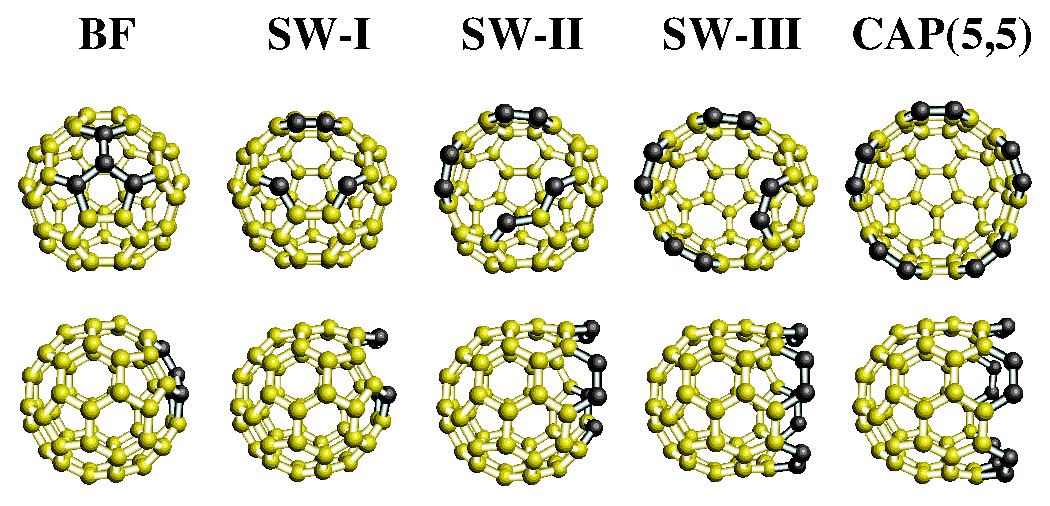
\includegraphics[width=12.5cm]{sample-fig1}}
    \caption[캡션제목 넣으십시오]{그림 제목을 넣으십시오.
    } \label{mag-fig1}
\end{figure}

\chapter{맺음말}

마지막은 맺음말로 하는 것을 권합니다.

\setcounter{chapter}{0}
\appendix
\makeatletter % Add
\renewcommand{\@chapapp}{Appendix} % Add
\renewcommand{\chaptername}{Appendix} % Add
\makeatother % Add

\chapter{Chapter Name}
This is a chapter.

%%
%% 참고문헌 시작
%% bibliography
%% 위는 보기이므로 학과 또는 논문의 특성에 맞게 조정 가능함. 다만, 참고문헌마다 충분한 정보가 들어 있어야 한다.
\begin{thebibliography}{00}

\bibitem{FD1} 박상우, \underline{동시 송수신 안테나를 두 개 쓰는 협력 인지 무선통신망에 알맞은 전 이중 통신}, 한국과학기술원 석사 학위 논문, 2016.

\bibitem{RVP1} 송익호, 박철훈, 김광순, 박소령, \underline{확률변수와 확률과정}, 자유아카데미, 2014.

\bibitem{ML1} 송익호, 안태훈, 민황기, \underline{인지 무선에서의 광대역 주파수 검출 방법 및 장치}, 특허등록번호 10-1494966, 2015년 2월 12일.

\bibitem{SOCA1} 호우위시, 이원주, 이승원, 안태훈, 이선영, 민황기, 송익호, “선형 판별 분석에서 부류안 분산 행렬의 영 공간 재공식화,” \underline{한국통신학회 2012년도 추계종합학술발표회}, 대한민국 고려대학교, 242-243쪽, 2012년 11월.

\bibitem{EF1} 민황기, 안태훈, 이승원, 이성로, 송익호, “비간섭 전력 부하 감시용 고차 적률 특징을 갖는 전력 신호 인식,” \underline{한국통신학회논문지}, 제39C권, 제7호, 608-614쪽, 2014년 7월.



\bibitem{FD2} S. Park, \textit{Full-Duplex Communication for Cooperative Cognitive Radio Networks with Two Simultaneous Transmit and Receive Antennas}, Master Thesis, Korea Adv. Inst. Science, Techn., Daejeon, Republic of Korea, 2016.

\bibitem{RVP2}  I. Song, J. Bae, and S. Y. Kim, \textit{Advanced Theory of Signal Detection: Weak Signal Detection in Generalized Observations}, Springer-Verlag, 2002.

\bibitem{ML2} I. Song, T. An, and J. Oh, \textit{Near ML decoding method based on metric-first search and branch length threshold,} registration no. US 8018828 B2, Sep. 13, 2011, USA. 

\bibitem{SOCA2} H.-K. Min, T. An, S. Lee, and I. Song, “Non-intrusive appliance load monitoring with feature extraction from higher order moments,” in \textit{Proc. 6th IEEE Int. Conf. Service Oriented Computing, Appl.,} Kauai, HI, USA, pp. 348-350, Dec. 2013.

\bibitem{EF2} I. Song and S. Lee, “Explicit formulae for product moments of multivariate Gaussian random variables,” \textit{Statistics, Probability Lett.,} vol. 100, pp. 27-34, May 2015.

\end{thebibliography}

%%
%% 사사 시작
%% Acknowledgement
%% 사사 작성은 선택사항임
% @command acknowledgement 감사의글
% @options [1 | 2 | 3 |4 ]
% - 1 : 본문과 감사의 글이 둘 다 한글일 때  | 2 : 본문은 한글인데 감사의 글이 영어일 때 | 3 :  본문과 감사의 글이 둘 다 영어일 때  | 4 : 본문은 영어인데 감사의 글이 % 한글일 때 

\acknowledgment[1]
언제나 저를 바른 길로 이끌어 주시는 송익호 교수님께 큰 고마움을 느낍니다.
끝으로 오늘의 제가 있을 수 있도록 사랑으로 키워 주신 가족들에게 감사드립니다.
저의 이 작은 결실이 그분들께 조금이나마 보답이 되기를 바랍니다.


%%
%% 약력 시작
%% Curriculum Vitae
%% 약력 작성은 선택사항임. 약력 내용도 알맞게 바꿀 수 있음
% @command curriculumvitae 이력서
% @options [1 | 2 | 3 |4 ]
% - 1 : 본문과 약력이 둘 다 한글일 때  | 2 : 본문은 한글인데 약력이 영어일 때 | 3 :  본문과 약력이 둘 다 영어일 때  | 4 : 본문은 영어인데 약력이 한글일 때 

\curriculumvitae[1]

    % @environment personaldata 개인정보
    % @command     name         이름
    %              dateofbirth  생년월일
    %              birthplace   출생지
    %              domicile     본적지
    %              address      주소지
    %              email        E-mail 주소
    % - 위 6개의 기본 필드 중에 이력서에 적고 싶은 정보를 입력
    % input data only you want
    \begin{personaldata}
        \name       {안 진 현}
        \dateofbirth{199x}{x}{xx}
        \birthplace {...}
        \address    { ...}
     \end{personaldata}

    % @environment education 학력
    % @options [default: (none)] - 수학기간을 입력
    \begin{education}
        \item[2007. 3.\ --\ 2009. 2.] 고등학교 (2년 수료)
        \item[2009. 2.\ --\ 2013. 8.] 한국과학기술원 수리과학과 (학사)
        \item[2013. 9.\ --\ 2016. 2.] 한국과학기술원 수리과학과 (석사)
    \end{education}

    % @environment career 경력
    % @options [default: (none)] - 해당기간을 입력
    \begin{career}
        \item[2013. 9.\ --\ 2016. 2.] 한국과학기술원 수리과학과 일반조교
    \end{career}

    % @environment activity 학회활동
    % @options [default: (none)] - 활동내용을 입력
%%    \begin{activity}
%%        \item J. Choi, \textbf{Yong-Hyun Kim}, K.J. Chang, and D. Tomanek,
%%             \textit{Occurrence of itinerant ferromagnetism in C/BN superlattice
%%             nanotubes}, 5th Asian Workshop on First-Principles Electronic
%%             Structure Calculations, Seoul (Korea), October., 2002.
%%    \end{activity}
%% 학회활동을 쓰고싶으시면, 이 문서와 클래스 문서의 학회활동 부분을 사용하십시오.

    % @environment publication 연구업적
    % @options [default: (none)] - 출판내용을 입력
    \begin{publication}
        \item J. Ahn, \textit{Analysis of Tail Probability of Interference at a Node in 2-dimensional Homogeneous Poisson Point Process}, Master Thesis, Korea Adv. Inst. Science, Techn., Daejeon, Republic of Korea, 2016.
    \end{publication}

  \label{paperlastpagelabel}     % <-- 추가 부분: 마지막 페이지 위치 지정	
%% 본문 끝
\end{document}
